% NeuralOS v2 — Branch B paper. arXiv-ready article class.
% Build:  make            (tectonic, or latexmk/pdflatex if installed)
% Figs:   make figs       (python3 + matplotlib; see figs/README.md)
% Gate:   make gate       (language rules of record — must pass)
\documentclass[11pt]{article}

\usepackage[margin=1in]{geometry}
\usepackage{amsmath,amssymb,amsthm}
\usepackage{booktabs}
\usepackage{graphicx}
\usepackage{microtype}
\usepackage{xcolor}
\usepackage[numbers,sort&compress]{natbib}
\usepackage[colorlinks=true,linkcolor=blue!60!black,citecolor=blue!60!black,urlcolor=blue!60!black]{hyperref}
\usepackage{url}

\newtheorem{theorem}{Theorem}
\newtheorem{remark}{Remark}

% Term of record (seal 3 + the adjudication ruling): the adaptation's
% downstream effects are UNATTRIBUTED PERTURBATION. The words "steers"
% and "editing" are banned everywhere except (i) the verbatim ISC-82
% quotation in Sec. 6 and (ii) the literature's own names in Sec. 8.
% Enforced by `make gate`.

\newcommand{\system}{\textsc{NeuralOS}}
\newcommand{\unattrib}{\emph{unattributed perturbation}}

\title{A Spiking Substrate That Reads and Round-Trips a Shipped
  Quantized LLM's Weights}

\author{%
  Caramoussin\thanks{Independent. Code and evidence:
  \url{https://gitea.com/Caramoussin/NeuralOs-v2} (AGPL-3.0).}%
}
\date{Draft of 2026-08-20\quad---\quad Branch B (paper-draft)}

\begin{document}
\maketitle

\begin{abstract}
% ABSTRACT-LAST: written in the final commit, once body language has
% settled. Skeleton (docs/PAPER_OUTLINE.md): substrate bullet carries
% the clamp caveat; adjudication is bullet 2; loop; surviving findings;
% method rungs.
% The abstract — written last, per the outline: the adjudication is
% bullet 2; the substrate bullet carries the clamp caveat.
We build a spiking substrate that reads, adapts, and round-trips the
weights of a shipped, quantized large language model: a
\texttt{no\_std}, \texttt{i16} fixed-point SNN library (LIF + STDP,
published on crates.io, byte-level test vectors against real
artifacts) whose ternary format bridge round-trips BitNet
\texttt{i2\_s} bit-exactly and a real 4B Q2\_0 LLM's tensor
two-way. Driven by the model's own activations (a sign-dominant drive
at this calibration --- 69.5\% of dim-steps railed at the clamp;
stated in-text), the substrate's firing \emph{tracks} the model's
weight arrangement over census (Hamming gap 1.35--1.36$\times$ under
the in-vivo drive, 1.63$\times$ synthetic; one slice, one model, one
seed --- a sensitivity result at $n{=}1$, not a population claim),
and local plasticity rewrites a declared $0.5\%$-of-one-layer
chunk of the shipped file, byte-audited and deterministic, which a
pinned foreign runtime (a llama.cpp fork) then executes; a
byte-identical control export rules out file-surgery artifacts.
\textbf{The adjudication, up front:} the adapted file does change
greedy continuations (2 of 5 frozen prompts, both on the
pre-registered low-margin subset) --- but those changes
\emph{failed every pre-registered criterion} for exceeding equal-dose
random perturbation (8 of 10 dose-matched nulls land the in-vivo
run's exact destination basin; margin shift 0.0798 vs.\ null-max
0.2254). The term of record is \emph{unattributed perturbation}:
the pre-registered null ladder --- committed before its authors could
see the null tables --- killed the authors' own earlier capability
reading before it could be published. The findings that stand are
infrastructure and method: the closed loop itself, the
arrangement-tracking sensitivity, the falsification-driven discovery
of a structural transmission bug and its mechanism reversal, a
counted clamp-rectified plasticity decomposition, a
composition-specific null-feasibility theorem proving content and
placement formally entangled at this terminal-diff composition, and
the destination-basin analysis that caught what flip-counts misread.

\end{abstract}

\section{Introduction}
\label{sec:intro}

Two research communities have arrived, independently, at the same
weight alphabet. Ternary large language models --- BitNet-class
systems shipped in $\{-1, 0, +1\}$ quantizations with integer
runtimes \citep{bitnet158,bitnnetcpp} --- put a three-symbol weight
world into production. Spiking neural networks compute natively in
that same integer regime, and their local, online plasticity rules
(STDP, Hebbian learning) update weights without backpropagation,
gradients, or loss-guided search. The literatures do not cite each
other, and --- as of this paper's surveyed date, with the field's own
surveys marking the gap open \citep{surveylargesnn,rajendran2023future} ---
no work has joined them: no published system applies local plasticity
to a shipped production LLM's weights.

This paper is the record of joining them, with the honesty that
turned out to require. We present \system{}, a
\texttt{no\_std} \texttt{i16} fixed-point spiking substrate whose
format bridge speaks the shipped ternary formats byte-exactly
(Sec.~\ref{sec:substrate}--\ref{sec:bridge}), and the closed loop it
enables (Sec.~\ref{sec:loop}): import a real 4B Q2\_0 LLM's weight
tensor into the spiking substrate, drive the substrate with
\emph{the model's own activations} (Sec.~\ref{sec:invivo}), let local
plasticity adapt the imported weights, re-export through the bridge
byte-exactly into a copy of the shipped file, and hand that file to a
pinned foreign runtime --- a llama.cpp fork --- which executes it.
Every step is deterministic and byte-audited; a control export
carries unadapted trits through the identical machinery and comes out
byte-identical to the original.

The loop closes. The adapted file measurably shifts the foreign
runtime's logits (60/60 generation steps at every judged footprint),
and the in-vivo-adapted file changes greedy continuations on 2 of 5
frozen prompts. The question that decides whether any of that is a
\emph{capability} is: do those changes carry the adaptation's
content, or would equal-dose random perturbation do the same? We
answered it with a pre-registered null ladder --- margin census,
dose-matched random families, a value-flip family, sibling prompts, a
report-only stress arm, three sealed rules --- committed in full
before any null table was read (Sec.~\ref{sec:adjudication}). The
verdict, by rule: the changes failed every pre-registered criterion.
Eight of ten equal-dose random perturbations land the in-vivo run's
exact destination. The term of record is \unattrib{}.

We report that negative as a first-class result for three reasons.
First, it was \emph{our} false positive to catch: the project's own
ledger, pre-adjudication, recorded the continuation change as a
capability demonstration (quoted verbatim in
Sec.~\ref{sec:averted}); only the pre-committed rule reversed the
authors' first reading. Flip-count evidence in this regime publishes
false positives. Second, the negative is structurally informative:
the model has generic destination basins that equal-dose noise
reaches at high probability, its knife-edges are fragile to
perturbation magnitude, and --- by a theorem this paper proves from
the terminal diff's composition --- content and placement are
formally entangled at this composition, so the natural control rung
does not exist (Sec.~\ref{sec:discussion}). Third, what survives is
exactly the infrastructure claim the title makes: a spiking substrate
that tracks a shipped quantized LLM's arrangement, adapts under its
own activations, and round-trips its weights through the production
format into foreign tooling --- first as surveyed, with the survey's
boundaries stated and the pre-submission re-verification standing as
a gate (Sec.~\ref{sec:related}).

\paragraph{Contributions.}
\begin{itemize}
\item \textbf{The substrate and bridge} (Sec.~\ref{sec:substrate},
  \ref{sec:bridge}): a published, \texttt{no\_std}, integer-only SNN
  library with byte-exact two-way ternary format bridges, and the
  falsification-driven discovery of a structural transmission bug
  whose fix reversed the substrate's plasticity mechanism ---
  a case study in pre-registered debugging inside infrastructure.
\item \textbf{The loop} (Sec.~\ref{sec:loop}--\ref{sec:invivo}): the
  L1--L4 chain closed on a shipped 4B Q2\_0 LLM --- local plasticity
  under the model's own drive, byte-audited re-export, foreign
  execution, control identity --- with the substrate's
  arrangement-tracking result under both synthetic and in-vivo drives
  (n=1, caveats in-text).
\item \textbf{The adjudication} (Sec.~\ref{sec:adjudication}): a
  pre-registered null ladder that refutes content-attribution at this
  composition and reports \unattrib{} --- including the two rungs we
  believe are novel: a composition-specific null-feasibility theorem,
  and destination-basin analysis, which together caught the false
  positive the authors' own first reading had become.
\end{itemize}

The remainder of the paper: Discussion of what would have counted and
why the negative informs (Sec.~\ref{sec:discussion}); related work and
the survey matrix (Sec.~\ref{sec:related}); limitations, pre-registered
(Sec.~\ref{sec:limitations}); destination transcripts and full
reproducibility material in the appendices.

\section{The substrate}
\label{sec:substrate}

The engine under everything that follows is \system{}, a
\texttt{no\_std} Rust spiking-neural-network library with an
\texttt{i16} fixed-point hot path (LIF neurons, STDP synapses, CSR
sparse connectivity), published as \texttt{neuralos-snn} on
crates.io. Integer-only computation is not an aesthetic choice: it is
the regime ternary weights live in natively (an \texttt{i16} state
holds a $\{-1,0,+1\}$ alphabet without conversion), and float-free SNN
computation has been independently motivated for FPU-less edge silicon
(IEEE 2025, \emph{Full-Integer SNN Inference with RISC-V ISA}). The
library forbids allocation and unwraps on the hot path; every number
in this paper is produced by that integer path.

\subsection{Two discretization grids, two dead zones}
\label{sec:grids}

Membrane potential integrates in integer units on one of two grids
(\texttt{VoltageResolution}): millivolt (the historical default) and
centi-millivolt (dead zone $\approx 2\,\mu$A), added when the mV
grid's quantization proved load-bearing. Each grid has a
\emph{per-type} dead zone for input currents (mV: $\sim$200\,$\mu$A
for E-cells, $\sim$100\,$\mu$A for I-cells) below which a single
pulse is absorbed without membrane movement. The climb barrier is
asymmetric and pinned by test: at a 300\,$\mu$A drive the membrane
sticks at $-59$\,mV; a $+12\,\mu$A recurrent pulse ratchets it
$+1$\,mV; a $-12\,\mu$A pulse is absorbed. Small weights are real
physics on these grids, not noise: whether a $\pm 12\,\mu$A pulse
moves the membrane is exactly the difference between the two grids,
and the paper's substrate claims are grid-keyed throughout.

\subsection{The population}
\label{sec:population}

All experiments in this paper use a 512-neuron slice of a real model
tensor --- 409 excitatory, 103 inhibitory, 261{,}632 directed pairs
--- with pair-based STDP ($\gamma = 125$), a fixed inhibitory wall
($I_{\mathrm{INH}} = 600\,\mu$A), and per-class raw/absorbed/applied
plasticity counters (Sec.~\ref{sec:mechanism}). Seeds are pinned;
every run is deterministic, and every claimed double-run produced
byte-identical exports.

\subsection{Case study: the dead wire, found by falsification}
\label{sec:deadwire}

The substrate's central debugging story is worth telling in full,
because it is the paper's clearest demonstration of
pre-registration paying for itself \emph{inside} the infrastructure,
months before the adjudication ladder did the same for the science.

\paragraph{Two pre-registered predictions, two falsifications.}
To test whether imported weights influence firing, we swept drive
amplitude with three nets --- imported weights, census-shuffled
control, zero --- and pre-registered the prediction that their spike
trains diverge at 600\,$\mu$A. Result: \textbf{honest NO} --- the
three trains were identical at \emph{every} amplitude (train Hamming
0, rate-L1 0, across the full 9-amplitude grid). A second, finer-ruler
sweep on the new centi grid (pre-registered again: divergence expected
once mV truncation stopped absorbing pulses) falsified the rescue
hypothesis too: totals shifted, E-cells fired at amplitudes the mV
grid had silenced --- and the trains remained identical.

\paragraph{The canary.}
Two falsified predictions forced a code re-read in place of a third
hypothesis, and the re-read found the structural cause:
\texttt{step()}'s Phase 2 injected the recurrent current
(\texttt{weight/10}) into the postsynaptic accumulator \emph{after}
Phase 1's integration, and the next step's opening loop called the
accumulator clear \emph{before} Phase 1 --- every recurrent pulse was
born and destroyed without ever reaching \texttt{integrate\_and\_fire}.
The canary test
(\texttt{recurrent\_current\_is\_never\_integrated\_in\_step\_bug\_pinned})
pinned it empirically: a 2-neuron net, the presynaptic cell fires, the
postsynaptic membrane never leaves $-70$\,mV. The wire had been cut
since the original port; the mV dead zone (real, unit-proven) had been
a co-blocker upstream of the cut. An earlier audit's claim that
``the pulse integrates with one-step delay'' was re-reading the code
comment's intent, not the code's behavior.

\paragraph{The fix and the shared miss.}
The fix reorders the step: adaptation-current decay $\to$ integrate
(reads the previous step's pulses --- the one-step delay the design
always claimed) $\to$ clear-after-read $\to$ propagate $\to$
plasticity. Exact-value tests pin transmission on both grids
(centi: $-7{,}000 \to -6{,}988$ exactly one step after the presynaptic
spike; mV: $-70 \to -68$ with a strong weight; two presynaptic spikes
sum their quanta). The chastening datum: the library's 152-test suite
was green before and after --- \emph{no unit pin had ever exercised
live transmission through \texttt{step()}}. The tests pinned the
parts; nothing pinned the wire between them.

\paragraph{The mechanism reversal.}
Re-running the import experiment on the live wire reversed the
substrate's plasticity mechanism. Dead-wire era: correlated pairs
drifted \emph{negative} (same-step co-fire tie-break LTD,
anti-Hebbian, $\Delta\mathrm{SI} = -1.0000$) --- an artifact of a
regime in which weights could not transmit. Live wire: pre spikes
causally drive post spikes one step later $\Rightarrow$
pre-before-post $\Rightarrow$ LTP: intra-class mean $\Delta$
flipped from $-0.3133$ to $+0.1075$, discrimination magnitude
$|\Delta\mathrm{SI}| = 1.0000$ in \emph{both} eras. The sign was
never the selectivity claim; it is the mechanism label. The frozen
gate's directional criterion --- written during the dead-wire era ---
read the post-fix result as COLLAPSES and parked the pipeline
honestly; the amended criterion asserts the raw non-degenerate fields
(intra $|\mathrm{mean}\,\Delta| \ge 0.05$, flips $>0$, Hamming
$<0.50$, zero sign crossings) and prints the direction as the era's
mechanism label.

\subsection{Arrangement vs.\ census}
\label{sec:arrangement}

With the wire live, the import experiment's question got a real
answer. On the centi grid at 600\,$\mu$A: imported vs.\ its own
census-shuffle control diverges far more than imported vs.\ zero ---
$H(i,c) = 39{,}011$ vs.\ $H(i,z) = 23{,}907 \approx H(c,z) =
23{,}958$ (1.63$\times$): \emph{firing reads the arrangement of the
model's weights, not just their census}. The mV grid tells the
complementary story: rate/Hamming sensitivity to weights (Hamming
58{,}779 at 600\,$\mu$A; recruitment at 300\,$\mu$A where imported
fires 1.14\,Hz, control 0.99, zero 0.00 --- coherent same-group
bursts stack past the shrunken margin; a Gaussian-$\sigma$ analysis
would have missed that bursts are coherent) --- with single weight
pulses dead-zone-absorbed. Under the model's own in-vivo drive the
same inequality holds at 1.35--1.36$\times$
(Sec.~\ref{sec:invivo}). Boundary, stated: one slice, one model, one
seed --- a sensitivity result, not a population claim.

\subsection{The mechanism label, counted}
\label{sec:mechanism}

The substrate's realized plasticity mechanism is not what the naive
Hebbian reading of Sec.~\ref{sec:deadwire} suggests --- and the
refutation came from the substrate's own counters. Cumulative
per-class counters ($\mathrm{raw} = \sum$ pre-clamp deltas;
$\mathrm{absorbed} = \sum$ clamped-away remainder; applied by
difference) decomposed the live-wire run: raw intra drift
$-739{,}295$ (mean $-17.85$/syn --- same-step and post-leads LTD
events dominate the raw stream) $\cdot$ clamp-absorbed $-839{,}029$
$\cdot$ \emph{applied} $+99{,}734$ (mean $+2.41$/syn). The realized
mechanism is \textsc{pairing-selective, clamp-rectified}: which pairs
drift is timing-driven (only co-firing pairs pair at all), but the
\emph{direction} of realized drift is bounds-driven --- the E-class
zero-floor absorbs the net-negative raw drift and the applied residue
potentiates. The examples compute the label from the counters (three
cases: raw-LTP-dominant $=$ Hebbian-carried; raw-negative with
applied-positive $=$ clamp-rectified; applied-negative $=$
LTD-carried); this is the decomposition the in-vivo runs of
Sec.~\ref{sec:invivo} inherit, and Fig.~\ref{fig:mechanism}
(Sec.~\ref{sec:loop}) sketches its two rectification stages.

\section{The format bridge}
\label{sec:bridge}

A substrate that cannot speak the shipping formats of the ternary
world is a simulation; this section is the part that makes it an
infrastructure claim. The bridge implements three wire formats, with
layouts pinned \emph{verbatim from reference source code} --- not
blogs, not model cards: BitNet \texttt{i2\_s} from
\texttt{microsoft/BitNet}'s conversion script (import and export),
and Prism \texttt{q1\_0}/\texttt{q2\_0} from the fork's
\texttt{ggml-common.h} and \texttt{ggml-quants.c} (import;
\texttt{q2\_0} two-way since the export codec landed). The
\texttt{q2\_0} layout was re-pinned from the fork source plus the
first real \texttt{q2\_0} file when the initial pin proved
incomplete --- layouts earn their pinning the hard way here.

\paragraph{One code table, three scale conventions.}
All three formats encode a trit in 2 bits with the same table
($00 \to -1$, $01 \to 0$, $10 \to +1$; $11$ unreachable-by-law,
below), LSB-first within each byte. The scales differ and travel as
\emph{raw bits}: \texttt{i2\_s} stores an f32's bits as a 32-byte row
tail (BitNet-Round $\gamma = \mathrm{mean}|w|$); \texttt{q1\_0}
stores fp16 bits per 128-weight block (the same $\gamma$ convention);
\texttt{q2\_0} stores fp16 bits with $d = \max|w|$ (TWN-style). The
library is integer-only, so fp16 scales are widened by
\texttt{half\_to\_f32\_bits} --- a pure-integer, bit-exact widening
--- and viewed in fixed point by \texttt{half\_to\_milli}
($\mathrm{round}(v \times 1000)$, saturating, NaN $\to$ 0, all
documented and tested).

\paragraph{The transposed packing.}
\texttt{i2\_s} does \emph{not} pack 4 sequential trits per byte. The
reference reshapes a 128-block into $4 \times 32$ lanes and packs lane
0 at bits 7--6, lane 1 at 5--4, lane 2 at 3--2, lane 3 at 1--0 of the
same 32 bytes: element $i$ lives at byte
$(i/128)\cdot 32 + (i \bmod 32)$, shift $6 - 2\lfloor (i \bmod
128)/32 \rfloor$. This trips up every hand-rolled decoder; it is
pinned here because it tripped up ours. The worked example in the
format spec is byte-identical to the crate's unit-test vector.

\paragraph{Byte identity, not almost.}
The round-trip claims are byte-level and tested against real
artifacts, not synthetic self-agreement:

\begin{itemize}
\item \texttt{i2\_s}: encode and decode are exact inverses; round-trip
  property tests over random tensors, plus the known-vector and
  golden-vector pins (decode$\,\circ\,$encode reproduces the pinned
  reference bytes).
\item \texttt{q2\_0} import on the real shipped file: a 253-block
  probe decodes byte-exactly against the fork's own reader
  (253/253), first block scale $0\mathrm{x}24\mathrm{c}8$ $=$ 18.68
  milli $\max|w|$, trit census $+37 / 0{\times}43 / -48$ of 128 ---
  the census the crate's tests still pin.
\item \texttt{q2\_0} export: the exact byte-level inverse of the
  decoder, re-using the file's original fp16 scale bits untouched
  (Sec.~\ref{sec:loop}); decode$\circ$encode $=$ byte identity on
  both pinned vectors, and code 3 (the value the reference quantizer
  cannot produce) is \emph{unconstructible} --- every lane is written
  from a \texttt{Trit}, so the encoder cannot emit the code the
  ecosystem would reject.
\end{itemize}

The bridge's discipline is the paper's in miniature: every layout is
pinned to a fetched reference source, every vector is real bytes from
a real shipped model, and every claim of exactness is a test that
would catch a one-bit drift.

\section{The loop: surgery, gates, control identity}
\label{sec:loop}

The bridge lets tensors out; the loop is the disciplined act of
putting them back into a shipped file. The surgery exports the
adapted $512\times512$ slice through \texttt{encode\_q2\_0} with the
file's \emph{original} fp16 scale bits passed through untouched --- a
recorded decision: the substrate adapted structure at $\gamma=125$;
magnitudes stay the model's own --- and splices the encoded blocks
into a copy of the GGUF as 512 disjoint 136-byte chunks (row $r$
occupies bytes $[r\cdot 680,\ r\cdot 680 + 136)$ of
\texttt{blk.0.attn\_q.weight}). Two details carry the safety of the
whole operation: the rows are \emph{non-contiguous} (680-byte stride,
136-byte payload --- a layout a pre-session audit caught before any
write), and the tensor window is computed from the file's dims, never
from inferred slice ends.

\paragraph{Two gates, asserted in-loop.}
\textbf{S1 (containment):} every differing code byte lies inside a
declared chunk --- outside-diffs $= 0$, scale bytes $= 0$, asserted
per row (synthetic-era run: 29,734 code bytes; in-vivo H2: 48,878).
\textbf{S2 (disk round-trip):} the written file re-parses as GGUF and
its 262{,}144 first-slice trits decode to \emph{exactly} the adapted
slice --- 0 mismatches. Determinism is structural: every double-run
in the record produced sha-identical patched files
($87078612\ldots$ synthetic era; $24\mathrm{ffe}5\mathrm{f}3\ldots$
Hebbian era; $71\mathrm{f}2518\mathrm{a}\ldots$ the in-vivo H2 export
of Sec.~\ref{sec:invivo}).

\paragraph{Control identity: the surgery is a measured transparent
transformation.}
Before any adapted export was judged, the pipeline ran end-to-end in
control mode --- decode, encode, splice, with \emph{unadapted} trits.
The written file equals the original, byte for byte (sha
$4\mathrm{e}0\mathrm{bf}8\mathrm{b}7\ldots$ on both). Whatever the
judge later measures, file-surgery artifacts are ruled out by
construction: the only difference between baseline and patched files
is the declared chunk content.

\paragraph{The judge protocol.}
The foreign runtime is a pinned fork of llama.cpp (commit
\texttt{9ca265a}, branch \texttt{prism}, clone HEAD $==$ pin
verified; the dump patch is env-gated, sits at the completion sample
site, and prints raw top-10 pre-sampler logits). Protocol: five
frozen prompts, greedy decoding forced, \texttt{-t 4}, \texttt{-n
12}, double-run per variant; every double-run in the record is
byte-identical. Instrument sanity first: the baseline run reproduces
the fork's previously recorded anchors exactly (p3 step-0 token
7794 at 14.6527; p2 step-0 token 4236 at 13.2278) --- the judge
measures the same logits the fork's own history measured.

\paragraph{What the loop showed, era by era.}
The synthetic-era closure (drive: a structured synthetic schedule):
\textbf{60/60} generation steps moved their logits (max $|\Delta|$
0.534 on p2; 0.452/0.124/0.093/0.088 on the others), top-10 overlap
8--10/10, \textbf{0/60} argmax flips, continuations byte-identical to
baseline --- at a footprint of $0.5\%$ of one layer across 36
measured layers. The Hebbian-era export (post transmission-fix,
Sec.~\ref{sec:substrate}) shifted logits on 60/60 steps again (max
$|\Delta|$ 0.42, mean 0.057--0.151), 0/60 flips. That is the loop's
standing sensitivity result at synthetic footprints: the foreign
runtime \emph{always} feels the substrate's write --- every judged
export moved logits on 60/60 steps --- while greedy continuations do
not change. The in-vivo writes (Sec.~\ref{sec:invivo}) break that
second half on 2 of 5 prompts; whether those changes carry adaptation
\emph{content} is precisely what Sec.~\ref{sec:adjudication}
adjudicates.

\section{In-vivo drive: the model's own activations}
\label{sec:invivo}

Everything up to here drove the substrate with synthetic schedules. The
question this section answers is whether the substrate still
\emph{tracks} --- and adapts under --- the shipped model's own activity:
the drive is $\mathrm{attn\_norm}(\mathrm{embedding})$ of a
sha-pinned corpus slice, captured from the model's own forward pass
(RMS-norm applied to the captured embeddings; no new dependencies).%
\footnote{Corpus: \texttt{evidence/corpus\_readme\_pinned.txt}, sha
$18\mathrm{fb}5452\ldots$ (12{,}148 bytes, 4{,}411 tokens). The
registration froze the entire drive protocol before any code ran
(ISA, session-H decision, 2026-08-19).}

\paragraph{Drive design (frozen pre-run).}
One token maps to one substrate step, so consecutive tokens present
causal pre$\to$post pairings at $\mathrm{dt}\approx1$\,ms (STDP factor
0.95). A per-step, per-dimension current
$I = \mathrm{clamp}(h_{\mathrm{dim}} \cdot k, \pm1000\,\mu\mathrm{A})$
injects into dimensions $0..408$ of the E population; the I population
keeps its validated fixed $I_{\mathrm{INH}}=600$ wall, so mechanism
attribution stays on validated ground. The single global gain $k$ is
set so corpus-wide RMS current lands mid-band
($\approx450\,\mu\mathrm{A}$). Deliberately rejected: an
$N$-steps-per-token mapping, which would manufacture sustained
same-step LTD --- the very mechanism the dead-wire era had run on only
as an artifact (Sec.~\ref{sec:substrate}). The grid is CENTI: the
arrangement-tracking result's only lineage is on that grid, and a
verbatim re-import on the mV build would absorb single weight pulses in
the dead zone and fail spuriously.

\paragraph{Two runs, one correction.}
The first run (H1) drove 6 whole epochs of the corpus head; its judge
results triggered a full audit that found a corpus infidelity --- the
run had consumed a 1{,}024-byte slice, not the pinned 12{,}148-byte
slice, because the registration's own constraints were mutually
unsatisfiable at the intended length and had been resolved silently in
code. The correction was a re-run (H2: first 2{,}000 of 4{,}411 tokens
in order, single truncated pass, no epochs, no wrap by construction),
not an annotation. We report both where they contrast, because H1 vs
H2 varies text, repetition, and gain together --- a confound by design
of the correction, with the de-confound arm (true corpus head $\times$
6 epochs) named as follow-on work. The head-bias this admits
(first-2{,}000 tokens of a README are not corpus statistics) is stated,
not hidden.

\begin{table}[t]
\centering
\caption{Tier-1 substrate gates under the in-vivo drive. $H(i,c)$:
spike-train Hamming between the imported-weights net and its
census-shuffle control; $H(i,z)$: imported vs zero-weights net.
G0 passes iff firing diverges from the arrangement-destroyed control
more than from the arrangement-free floor. Rate-L1 agrees in both
runs.}
\label{tab:t1gates}
\begin{tabular}{lcccc}
\toprule
 & $H(i,c)$ & $H(i,z)$ & ratio & rate-L1 ($i,c$ vs $i,z$) \\
\midrule
H1 (6 epochs) & 41{,}190 & 30{,}216 & 1.36$\times$ & 1{,}440 vs 1{,}040 \\
H2 (single pass) & 41{,}555 & 30{,}724 & 1.35$\times$ & 1{,}309 vs 950 \\
\bottomrule
\end{tabular}
\end{table}

\paragraph{Tier 1: the substrate tracks arrangement under the model's
own drive.}
Table~\ref{tab:t1gates} gives the gate results. G0 --- firing tracks
model arrangement over census --- passes in both runs, with the
metric battery (pairwise train Hammings, per-neuron rate-L1,
per-population Hz) agreeing throughout; the wire-liveness tripwire
(weights borne in spike trains) also passes. The pre-registered
prediction P1$'$ had teeth: if the single-pass correction weakened the
arrangement signal, the H2 gap $H(i,c)-H(i,z)$ had to stay above
$\approx$25\% of H1's 10{,}974 (floor 2{,}744). Observed: 10{,}831
--- 98.9\% of H1's gap. Single-pass does not weaken G0. We note the
boundary honestly: this is one slice of one model under one seed, a
sensitivity result on the centi grid, not a population claim.

\paragraph{The clamp caveat (stated in-text, per the registration).}
The registration demanded a clamp audit, and it fired hard:
69.80\% of dim-steps (H1) and 69.48\% (H2: 568{,}321 of 818{,}000)
railed at $\pm1000\,\mu\mathrm{A}$; the hottest dimension (dim 199)
railed on 89\% of its steps (H2) / 90\% (H1). Post-RMSNorm activations
are far heavier-tailed than the corpus RMS, so the \emph{effective}
drive is sign-dominant, not amplitude-graded --- ``amplitude-informed''
is not what ran. The gates above pass on a \emph{shared} drive (both
the imported and control nets see the same railed currents), so the G0
contrast stands; but any claim that the substrate exploited
fine-grained activation \emph{magnitudes} would overstate the
protocol. Per-dimension standardization is the named fix, not applied
here.

\paragraph{The class structure dissolves under real co-firing.}
Second honesty flag, recorded per the registration itself: the
4-group intra/inter class structure that the synthetic schedule
produced \emph{dissolved} under data-driven co-firing. In H1,
inter-class applied drift went \emph{positive} too (mean $\Delta$
+0.0777 inter vs +0.0606 intra --- inverted against the synthetic
era); in H2 both classes potentiate (intra +0.0805 over 41{,}412
pairs, inter +0.0976 over 220{,}220). The model's own activity treats
the slice as one co-active assembly, not four groups:
class-selectivity observations from the synthetic regime do not
transfer.

\paragraph{Adaptation under in-vivo drive.}
With STDP on ($\gamma=125$), firing sustains at 43.93\,Hz (H1) /
43.65\,Hz (H2); H2 logs 25{,}302{,}899 events and 1{,}112{,}771 weight
flips, Hamming distance to the imported state: 87{,}119 of 261{,}632
(33.30\%; H1: 25.73\% on 6$\times$-repeated text ---
more text diversity, more drift). Pairing was perfectly symmetric
(post-leads $=$ pre-leads $=$ 7{,}030{,}561), and the mechanism label
--- \textsc{pairing-selective, clamp-rectified}, exactly as
pre-registered-expected --- matches the post-fix substrate physics:
net-negative raw drift, zero-floor absorption, applied residue
potentiates (Sec.~\ref{sec:substrate}). Export checkpoints are
monotone in dose (61{,}210 $\to$ 71{,}381 $\to$ 80{,}391 $\to$ 87{,}119
changed cells), every export re-reads clean through the format bridge,
and the 100\%-checkpoint export is asserted byte-identical to the plain
export (sha $71\mathrm{f}2518\mathrm{a}\ldots$) --- the checkpointing
machinery itself perturbs nothing. Both runs are deterministic:
independent double-runs produce byte-identical exports.

The artifact that exits this section --- a shipped-quantized LLM whose
declared chunk was re-written by the model's own activity flowing
through a spiking substrate --- is exactly the artifact whose
downstream behavioral fate the next section adjudicates.

\section{The adjudication: unattributed perturbation}
\label{sec:adjudication}

Section~\ref{sec:invivo} delivered the artifact; this section delivers
its verdict. The in-vivo-adapted file changes greedy continuations on
2 of 5 frozen prompts (both on the pre-registered low-margin subset),
and the question this section answers was fixed before any of it was
observed: \emph{are those changes attributable to the adaptation's
content, or would equal-dose random perturbation do the same?} The
answer, by a pre-registered decision rule, is the second. The term of
record for the adaptation's downstream effects is
\unattrib{}. This section shows the ladder that produced that ruling
--- and the false positive it caught, which was ours.

\subsection{The decision rule (committed before the evidence)}
\label{sec:rule}

The sequence of commitments is itself part of the method, and the
dates bind: the five judge prompts were frozen first; then a margin
census over every prompt$\times$step of the baseline dumps defined the
knife-edge set (top1$-$top2 margin $< \theta = 0.05$, keyed on
\emph{baseline} margins --- model properties before perturbation; the
patched side is an outcome, never a key); only then were the null
families generated and judged. Sibling prompts (weekday-triple
rotations, a month chain, length-matched off-circuit negatives, a
digit run) were rule-fixed before running, evidence-only.

The pre-registered conjunct: content-attribution survives \emph{only
if} all four arms hold ---
\begin{enumerate}
\item[(a)] the continuous statistic, $|\Delta\mathrm{margin}|$ at every
  knife-edge, for the in-vivo file exceeds the maximum over
  \emph{all} nulls;
\item[(b)] the null flip-rate on the knife-edge set is $\le 1/10$
  (escalation to $n{=}20$ at $0$--$1/10$, since the rule-of-three
  confidence interval at $n{=}10$ is too wide to carry the claim
  alone);
\item[(c)] the in-vivo dose curve exits the null band
  (mean\,$\pm$\,2SD) at every checkpoint;
\item[(d)] effects concentrate on the weekday set vs.\ off-circuit
  negatives.
\end{enumerate}
Any arm failing demotes the capability language --- recorded, not
debated.

\subsection{The null ladder}
\label{sec:ladder}

\paragraph{Primary family: dose-matched $\times$10.}
Each of ten draws changes \emph{exactly} 87{,}119 cells --- the H2
terminal dose --- with positions and values sampled from the H2
terminal diff (decoded from the patched artifact itself, never
re-run), region-matched, i.i.d.

\paragraph{The rung that cannot exist.}
The original design included a position-shuffle rung: keep H2's
changed-cell set, permute the assigned new-values (isolating content
from placement). Building it found a structural impossibility.

\begin{theorem}[Composition-specific null-feasibility]
\label{thm:shuffle}
H2's terminal diff has value multiset $\{0^{\,57{,}170},
+1^{\,29{,}949}\}$ --- it contains no $-1$s. Under the no-same-source
constraint (a permuted value must differ from its source), the
feasible assignment polytope is a single point: the 0-sourced demand
($29{,}949$) equals the entire $+1$ pool, forcing
$x[0\!\to\!+1] = 29{,}949$ and exhausting it; $-1$-sourced cells can
then only take 0s ($26{,}027$ forced); $+1$-sourced cells take the
remaining 0s ($31{,}143$ forced). H2's own mapping is the unique legal
assignment.
\end{theorem}

Empirical confirmation: a pairwise-exchange search returns zero legal
swaps; a greedy shuffle implementation produced a file
byte-identical to H2 (caught by sha before judging); a randomizing
implementation grinds forever on dead-end restarts. The consequence is
banked as a finding about the regime, not a workaround: \emph{at this
composition, content and placement are formally entangled} --- no
value-permutation null exists, and any future claim to separate what
was changed from where must first exit this composition. The rung was
redefined, pre-registered before any null table was read, as
\emph{value-flip $\times$3}: the real changed positions at exact dose,
each new value reflected where legal ($-1\!\to\!0$ becomes
$-1\!\to\!+1$, $+1\!\to\!0$ becomes $+1\!\to\!-1$;
$0\!\to\!+1$ has no legal reflection and stays) --- testing ``the
specific values matter,'' while changing the value multiset by design.

\paragraph{Stress arm (report-only).}
The project's first null family was census-matched to
\emph{transition} totals (1{,}112{,}771 flips $\approx$ 178k cells ---
flips are not cells; the terminal patch is 87{,}119). Discovered by
pre-mortem, it is relabeled a $\approx$2$\times$-dose stress arm:
context in the figures, never adjudication.

\subsection{The seals}
\label{sec:seals}

Three rules were sealed before the primary family's tables were read,
eliminating every remaining discretionary surface:
\begin{itemize}
\item \textbf{Seal 1 (void protocol):} a void is mechanical evidence
  only (non-zero exit or empty dump); re-run once; void twice
  $\to$ excluded with the denominator adjusted. The primary family
  recorded zero voids. (The stress arm's r10--p3 was void under this
  protocol --- warmup death --- correcting its banked table to 8/9
  valid.)
\item \textbf{Seal 2 (p4 bands):} $0$--$1/10$ dose-matched p4 flips
  $=$ thresholded; $\ge 5/10$ $=$ content-evidence; $2$--$4/10$ $=$
  MIXED --- reported, no p4 claim either way.
\item \textbf{Seal 3 (language pre-adjustment):} capability wording
  pre-weakened in the paper skeleton for \emph{both} outcome branches,
  so the ruling could not be felt in the prose.
\end{itemize}

\subsection{The primary family's evidence}
\label{sec:primary}

\begin{figure}[t]
\centering
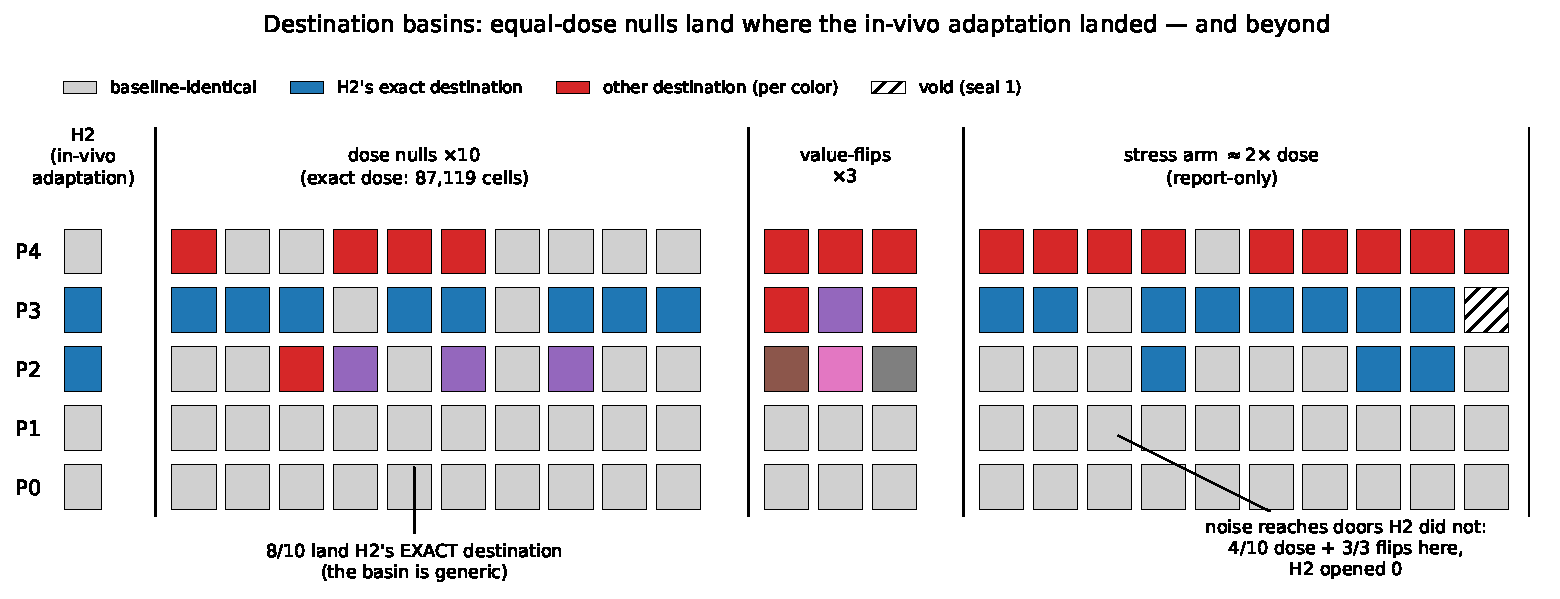
\includegraphics[width=\linewidth]{figs/basins.pdf}
\caption{Destination basins. Rows: judge prompts. Columns: the H2
(in-vivo) file, the ten dose-matched nulls, the three value-flip
nulls, and the report-only stress arm. Grey $=$ baseline-identical;
blue $=$ byte-identical to H2's continuation; other colors $=$ other
destinations; hatched $=$ void (seal 1). Eight of ten dose nulls land
H2's \emph{exact} p3 destination --- the basin is generic. Noise also
reaches doors H2 did not open (p4).}
\label{fig:basins}
\end{figure}

Figure~\ref{fig:basins} shows every draw's fate; the numbers here are
the README-recorded table the figure asserts against.

\paragraph{Flip counts.}
p0/p1: quiet everywhere (0/10, 0/3). p3: 8/10 dose nulls flip ---
\emph{and all eight land H2's exact destination} (``\,'Thursday' plus
ten newlines). p2: 4/10 (d3, d4, d6, d8). p4: 4/10 (d1, d4, d5, d6)
--- a MIXED band under seal 2: reported, no claim. Value-flips: p2
3/3, p3 3/3, p4 3/3.

\paragraph{Destinations --- p2's full denominator.}
The four dose-null p2 flips do \emph{not} form a degradation blob;
each destination is legible:
\begin{itemize}
\item \textbf{d3}: ``\ldots eleven twelve fifteen seventeen twenty
  one'' --- a \emph{different coherent odd chain}, not noise-salad;
\item \textbf{d4, d6, d8}: ``\ldots nine ten\,$\backslash$n\,What is
  the sum of'' --- the prompt's own trained continuation (the
  dead-wire-era basin), one line each; transcripts in
  Appendix~\ref{app:transcripts}.
\end{itemize}

\paragraph{The continuous statistic.}
At p3's step-1 knife-edge, H2 crosses the edge (margin $+0.0091 \to
-0.0707$) with $|\Delta\mathrm{margin}| = 0.0798$. The maximum over
all dose nulls at the same edge is $0.2254$ (null d6). Arm (a):
\textbf{FAIL} --- $0.0798 < 0.2254$. Arm (b): \textbf{FAIL} decisively
--- 8/10 null flips against a $\le 1/10$ bar; escalation is moot.
Arm (c): moot. Arm (d): MIXED per seal 2. The conjunct fails.

\subsection{The ruling}
\label{sec:ruling}

Branch B, by rule, zero discretionary calls: the in-vivo
adaptation's downstream effects fail every pre-registered criterion
for exceeding equal-dose random perturbation. \unattrib{} is the term
of record --- and two neighboring terms are explicitly refused:
\emph{degradation} is killed by d3's coherent chain (random
perturbation produced a \emph{different orderly continuation}, so
``degrades the model'' is not what random-walk-into-basins does), and
\emph{statistically indistinguishable} is refused because it claims an
unpowered equivalence this design never tested: the claim failed
pre-registered criteria, which is a refutation, not a tie.

Two footprint facts frame the ruling. H2's per-prompt footprint
$\{p2, p3\}$ sits \emph{inside} null experience --- noise reached
$\{p2, p3, p4\}$ (quantified in Sec.~\ref{sec:discussion}). And the
value-flips opened p4 3/3 where H2 opened 0 --- hypothesis-generating
only (the family changes the value multiset by design), but a pointer
to where content, if it exists, would have to show.

\subsection{The false positive we almost published}
\label{sec:averted}

The strongest evidence for the ladder is what it caught: us. The H1
run's judge result --- 11/12 argmax flips on the weekday prompt, a
complete continuation divergence after the shared first token --- was
recorded in the project's ledger, pre-adjudication, as:

\begin{quote}\small
``(i) STEERING demonstrated --- Tier-3's named stretch, achieved %%ALLOW%%
without widening'' %%ALLOW%% (verbatim quotation of the pre-adjudication reading; the term is retired)
\hfill --- project ledger, ISC-82, 2026-08-19
\end{quote}

Under the flip-count reading, that entry was a capability claim: the
in-vivo adaptation had moved the weekday prompt's dynamics decisively,
and four prior synthetic-era runs had shown 0/60 flips at this
footprint. The ladder then showed what the flips were made of: at
equal dose, random perturbation lands the same destination 8 times out
of 10. Flip-counts alone would have published a false positive; the
authors' first reading \emph{was} that false positive, and only the
pre-registered rule --- committed before the authors could see the
null tables --- reversed it. We report this openly because it is the
sharpest available demonstration of why the ladder's rungs (null
feasibility, destination basins, continuous statistics) are not
ceremony: they are what stands between a compelling count and a true
one.

\section{Discussion}
\label{sec:discussion}

\paragraph{What would have counted as content.}
The ruling of Sec.~\ref{sec:adjudication} is only as meaningful as
the result it refused, so we state the conjunct's positive side
concretely. Content-attribution would have required all four arms at
once: the in-vivo file's margin shift at every knife-edge exceeding
the worst null (here $0.0798$ vs.\ $0.2254$); the null family quiet on
the knife-edge set at $\le 1/10$ (here $8/10$); the in-vivo dose
response leaving the null band at every checkpoint; and effects
concentrated on the weekday circuit against off-circuit negatives.
The design could have produced that outcome --- the arms are
contingent facts about basins, not tautologies --- which is what makes
the negative informative rather than vacuous.

\paragraph{Why the negative is informative: three structural facts.}
First, \emph{basins}. The model's prompt-neighborhood has stereotyped
destinations, and an equal-dose random walk lands in them at high
probability (8/10 into H2's exact p3 continuation). Continuation
changes at this dose are therefore weak evidence about \emph{what}
caused them; only a destination (or statistic) that noise cannot reach
would be. Flip-counts read ``reproduces the signature'' where the
truth is ``reproduces the basin'' --- the distinction our own first
reading missed (Sec.~\ref{sec:averted}).

Second, \emph{dose}. The stress arm shows the p3 knife-edge is
fragile to perturbation \emph{magnitude}: at $\approx$2$\times$ dose,
i.i.d.\ noise of this composition flips it 8/9 (with the ninth void).
Attribution questions at one dose sit inside a landscape where
magnitude alone moves the observed quantity substantially.

Third, \emph{entanglement}. Theorem~\ref{thm:shuffle} is not a
technicality: at this terminal-diff composition, content and placement
are formally inseparable --- no value-permutation null exists, so
``the same cells, different values'' is not even definable without
exiting the composition (a terminal diff containing $-1$s, or scale-bit
changes, would restore the rung). Any future content claim on this
artifact class must either face that or engineer around it.

\paragraph{One quantified footprint sentence --- and its boundary.}
Pooling the primary family's per-prompt flip rates, a single
equal-dose noise draw opens at least H2's footprint $\{p2, p3\}$ ---
and p4 besides --- with probability $0.4 \times 0.8 \times 0.6 \approx
19\%$. We present this as context, not a claim: the per-prompt rates
come from pooling ten draws, so the product prices a single draw
against a union of ten --- the comparison that motivated cutting the
stronger ``noise reaches more doors'' reading from this paper's claims.

\paragraph{The honest boundary of the capability claim.}
What stands after the adjudication is exactly the outline of
Sec.~\ref{sec:invivo}--\ref{sec:loop}: a closed, deterministic,
byte-audited pipeline in which a shipped quantized LLM's declared
weight chunk is re-written by local plasticity under the model's own
activations and re-executed by foreign tooling, with control identity
and containment asserted in-loop --- and in which the resulting
behavioral changes are, by pre-registered rule, \unattrib{}. The
substrate's arrangement-tracking result (one slice, one model, one
seed) and the loop's 60/60 logit sensitivity are measured facts. What
we do \emph{not} have is evidence that the adaptation's content ---
as opposed to its dose --- drives anything the judge can see.

\paragraph{What the method costs, and buys.}
Pre-registering the ladder before the authors could see the null
tables is clinical-trial practice, imported whole: sealed void
protocol, pre-stated bands, pre-weakened language, a mechanical
ruling. The cost was real (the capability reading died by our own
rule). The buy is the paper's sharpest result: the demonstration,
on ourselves, that flip-count evidence in this regime publishes false
positives, and that a two-rung null ladder --- feasibility first,
destination basins second --- catches what neither intuition nor
counts catch. We suspect this regime property is not specific to
spiking substrates; any local, dose-heavy adaptation of a fragile
quantized model faces the same basin statistics.

\section{Related work}
\label{sec:related}

The novel intersection this paper occupies is the conjunction
L1$\wedge$L2: \allowbreak \emph{local, online plasticity} (STDP/\allowbreak
Hebbian class --- no backpropagation, no gradient, no loss-guided search) applied to
\emph{a pretrained production LLM's weights}. The export (L3) and
foreign-execution (L4) links are presented as closure of a chain, not
as novelty: the ternary ecosystem ships both natively. The field's
own literature marks the seam open: the large-SNN survey
\citep{surveylargesnn} lists only ANN$\to$SNN conversion and
surrogate-gradient backpropagation as training paradigms, and
\citet{rajendran2023future} name backprop-free on-device learning as
a \emph{future} neuromorphic principle; a 2025 SNN--LLM survey
reaches the same gap independently.

We verified the seam with three survey passes (2026-08-18/19/20:
arXiv, DuckDuckGo, direct fetches; OpenReview V1 API at
3$\times$1{,}000-note depth; OpenAlex precision queries; Semantic
Scholar citation graphs on the three nearest anchors; GitHub repo
search). Full query logs and boundaries are in the repository's
novelty document; the pass-3 verdict --- \emph{no L1$\wedge$L2
conjunction found} --- is the pre-submission gate this paper's
timestamp claim rests on. Table~\ref{tab:matrix} is the resulting
matrix, every entry fetched at the source.

\begin{table*}[t]
\centering
\caption{The L1--L4 matrix (pass 1: 2026-08-18, entries 1--16;
pass 3: 2026-08-20, entries 17--25). Every entry was fetched and read
at its source. \checkmark$=$ link present, $\sim$ $=$ partial, 
$\times$ $=$ absent. No entry satisfies L1$\wedge$L2.}
\label{tab:matrix}
\footnotesize
\setlength{\tabcolsep}{4pt}
\begin{tabular}{@{}c>{\raggedright\arraybackslash}p{60pt}>{\raggedright\arraybackslash}p{92pt}>{\raggedright\arraybackslash}p{78pt}>{\raggedright\arraybackslash}p{92pt}>{\raggedright\arraybackslash}p{78pt}@{}}
\toprule
\# & Work & L1 local plasticity & L2 shipped LLM & L3 quant re-export & L4 foreign run \\
\midrule
1 & SpikeGPT \citep{spikegpt} & $\times$ (BPTT, self-described) & $\times$ scratch & $\times$ & $\times$ \\
2 & SpikeLLM \citep{spikellm} & $\times$ (conversion in OmniQuant/GPTQ) & \checkmark\ 7--70B & $\times$ W4A4 own & $\times$ \\
3 & SpikingBERT \citep{spikingbert} & $\times$ (implicit diff + distill.) & $\times$ & $\times$ & $\times$ \\
4 & Bal et al.\ \citep{bal2024sparsellm} & $\times$ distillation & $\times$ & $\sim$ own 1/1.58-bit, GLUE-scale & $\times$ \\
5 & Dragon Hatchling \citep{dragonhatchling} & \checkmark\ Hebbian spiking & $\times$ scratch GPT-2-class & $\times$ & $\times$ \\
6 & Chaudhary \citep{chaudary2025} & \checkmark\ neuromod.\ Hebbian fast weights & $\times$ toy scratch & $\times$ & $\times$ \\
7 & Bio-Inspired Mamba \citep{biomamba} & $\sim$ STDP-like + RTRL & $\times$ & $\times$ & $\times$ \\
8 & S$^2$TDPT \citep{s2tdpt} & \checkmark\ STDP attention & $\times$ CIFAR vision & $\times$ & $\times$ \\
9 & EMBER \citep{ember} & \checkmark\ STDP+reward SNN & $\times$ LLM frozen, untouched & $\times$ & $\times$ \\
10 & AlphaEdit \citep{alphaedit} & $\times$ offline null-space LSQ %%ALLOW%% (field's own name; not our term)
  & \checkmark & $\times$ fp & $\times$ \\
11 & In-Place TTT \citep{inplacettt} & $\times$ gradient inner loops & \checkmark & $\times$ & $\times$ \\
12 & MeZO-class ZO tuning \citep{mezocluster} & $\times$ global loss-guided search & \checkmark & $\times$ & $\times$ \\
13 & QES \citep{qes} & $\times$ evolution strategies & \checkmark & $\sim$ PTQ INT4/8, in-place & $\sim$ vLLM via own harness \\
14 & CAT-Q \citep{catq} & $\times$ calibration PTQ & \checkmark\ 14B--235B$\to$ternary & $\sim$ no GGUF/i2\_s bridge & $\times$ \\
15 & BitDistill \citep{bitdistill} & $\times$ BP distillation & $\sim$ converts FP$\to$1.58-bit & $\sim$ bitnet.cpp-class & $\sim$ bitnet.cpp \\
16 & llama.cpp finetune \citep{llamacpp} & $\times$ ggml autodiff $=$ BP & $\sim$ & \checkmark\ in-GGUF & $\times$ same toolchain \\
\midrule
17 & Antahkarana \citep{antahkarana} & $\times$ LoRA+BP & \checkmark\ Phi-2 & $\times$ & $\times$ \\
18 & Photograph-STDP \citep{photographstdp} & $\times$ STDP on records, weights frozen & $\sim$ & $\times$ & $\times$ \\
19 & Spike-Aware C++ INT8 \citep{spikeaware} & $\times$ inference only & $\times$ scratch & $\sim$ INT8 own & $\sim$ own runtime \\
20 & NEXUS \citep{nexus} & $\times$ STE conversion & $\sim$ converted 70B & $\times$ & $\sim$ neuromorphic HW \\
21 & NSLLM \citep{nsllm} & $\times$ conversion+PTQ & $\sim$ 1.5B & $\sim$ & $\sim$ own FPGA \\
22 & QSLM \citep{qslm} & $\times$ automated PTQ & $\times$ scratch & \checkmark\ own & \checkmark\ embedded \\
23 & Kirin \citep{kirin} & $\times$ ANN$\to$SNN & $\sim$ & $\sim$ & $\sim$ \\
24 & WTA-Spikingformer \citep{wtaspikingformer} & $\times$ WTA$=$attention, surrogate BP & $\times$ & $\times$ & $\times$ \\
25 & BitRL \citep{bitrl} & $\times$ RL global reward (QES-class) & \checkmark & $\sim$ 1-bit & $\times$ \\
\bottomrule
\end{tabular}
\end{table*}

\paragraph{The three nearest neighbors.}
\textbf{QES} \citep{qes} holds L2 and half of L3/L4 --- quantized-space
adaptation of PTQ models with vLLM serving --- but its search is a
global evolutionary loss loop, not local online plasticity, and the
portable GGUF-class export is absent. \textbf{Dragon Hatchling}
\citep{dragonhatchling} holds L1 --- Hebbian spiking plasticity inside
an LLM --- on a scratch GPT-2-class model where plasticity acts as
transient working memory, not weight adaptation. \textbf{BitDistill +
bitnet.cpp} \citep{bitdistill,bitnnetcpp} proves our L3/L4 half
exists natively for ternary weights ($i2_s$, foreign CPU runtime);
its adaptation is BP distillation/QAT throughout. The nearest
knowledge-modification lines --- the locate-then-modify family
\citep{alphaedit}, test-time training \citep{inplacettt}, zeroth-order
tuning \citep{mezocluster} --- are gradient- or search-driven by
construction and stop before portable re-export; they are the ladder's
natural comparison class for adjudication design, not competitors on
the seam.

\paragraph{Supporting signal.}
The 447-citation graph of BitNet b1.58 \citep{bitnet158} contains
zero plasticity-titled successors; the large-SNN survey
\citep{surveylargesnn} lists no local-plasticity training paradigm at
LLM scale; \citet{rajendran2023future} mark the capability as future
work. The seam is open in the field's own record, independently of
this survey.

\paragraph{Boundaries of the survey, stated.}
Semantic Scholar search was throttled (13/14 requests 429; one
success logged; citation endpoints usable at $\sim$1
request/80\,s); OpenReview V2 search was unavailable (V1 covered at
3$\times$1{,}000 relevance depth per term); GitHub \emph{code}
search returned 401. A paper with no arXiv mirror at a closed venue
could escape this net --- priced low under the arXiv-first
convention, but nonzero. The seam claim is ``first as surveyed,
2026-08-20, boundaries stated,'' and the pre-submission re-pass is a
standing gate.

\section{Limitations}
\label{sec:limitations}

The boundaries below were written before, during, and after the
adjudication as standing armor --- most pre-date the results they
bound.

\paragraph{Sample size.} One slice (512$\times$512 of one tensor), one
model (a 4B Q2\_0 LLM), one seed per run. The substrate's
arrangement-tracking claim is a sensitivity result on that single
configuration; replicates $\times$3 were scoped ($\sim$25\,h wall),
deferred, and would upgrade the substrate and sensitivity claims
without being able to resurrect the adjudicated one. The n=1 caveat
is load-bearing for every measured claim in this paper.

\paragraph{The confounded correction.} H1 vs.\ H2 varies text
(1\,KB$\to$12\,KB corpus), repetition (6$\times\to$1$\times$), and
gain together --- by design of the corpus-infidelity correction, not
by accident. The de-confound arm (true corpus head $\times$ 6 epochs)
is named and unrun.

\paragraph{Sign-dominant drive.} 69.5--69.8\% of dim-steps railed at
the clamp (Sec.~\ref{sec:invivo}); the effective drive is
sign-dominant. Per-dimension standardization is the named, unapplied
fix; amplitude-graded claims are not available on this protocol.

\paragraph{Null-family boundaries.} The value-flip family changes the
terminal diff's value multiset \emph{by design} (reflection where
legal) --- it tests value-sensitivity, not a uniform permutation; the
uniform-permutation rung does not exist at this composition
(Thm.~\ref{thm:shuffle}). The stress arm's $\approx$2$\times$ dose is
census-matched approximation, report-only by pre-registration.

\paragraph{Judge scope.} Greedy decoding only, 12 generated tokens,
five frozen prompts, one pinned foreign runtime (fork commit
\texttt{9ca265a}; version-bump robustness untested --- named
follow-up). KLD breadth across corpora was scoped and dropped.
Continuation-level claims are bounded by exactly this protocol.

\paragraph{Footprint.} The declared chunk is $0.5\%$ of one layer of
36; wider exports were a named follow-on contingent on a capability
verdict, which the adjudication refused --- the widening question is
now moot for this paper and open for whoever resumes it.

\paragraph{Survey boundaries.} The seam claim is ``first as
surveyed,'' with the engine gaps stated in
Sec.~\ref{sec:related}; the re-verification gate stands.

\paragraph{What the negative does not mean.} The adjudication refutes
content-attribution \emph{at this composition, dose, and protocol} ---
it does not establish that local plasticity cannot carry content in a
quantized LLM, and the entanglement theorem shows this artifact
cannot even pose the placement-vs-content question without exiting
its composition. Both boundary statements are the pre-registered
armor, applied verbatim.


\appendix
\section{Destination transcripts (p2, p3)}
\label{app:transcripts}

Verbatim continuations (12 tokens, greedy, final newline rendered as
$\langle\backslash$n$\rangle$), byte-identical across double-runs.
Source files: \texttt{evidence/…/*\_run1.log} in the repository.

\paragraph{p3 --- the generic basin.}
\begin{tabular}{@{}ll@{}}
\toprule
baseline & Monday Tuesday Wednesday Thursday04/05/2018 \\
H2 (in-vivo) & Monday Tuesday Wednesday Thursday
$\langle\backslash$n$\rangle^{\times10}$ \\
dose nulls d1/d2/d3/d5/d6/d8/d9/d10 & Monday Tuesday Wednesday
Thursday $\langle\backslash$n$\rangle^{\times10}$ \\
dose nulls d4/d7 & Monday Tuesday Wednesday Thursday04/05/2018 \\
value-flips f1/f3 & Monday Tuesday Wednesday Thursday04:00~PM
$\langle\backslash$n$\rangle$The following is a \\
value-flip f2 & Monday Tuesday Wednesday Thursday04:00~PM 10:0 \\
stress arm (8/9 valid) & Monday Tuesday Wednesday Thursday
$\langle\backslash$n$\rangle^{\times10}$ \\
\bottomrule
\end{tabular}

\medskip
\paragraph{p2 --- the full denominator of the 4/10 dose flips.}
\begin{tabular}{@{}ll@{}}
\toprule
baseline & one two three four five six seven eight nine ten eleven
twelve thirteen fifteen fifteen seventeen \\
H2 (in-vivo) & one two three four five six seven eight nine ten
eleven twelve fifteen seventeen seventeen eighteen \\
dose null d3 & one two three four five six seven eight nine ten eleven
twelve fifteen seventeen \textbf{twenty one} \\
dose nulls d4/d6/d8 & one two three four five six seven eight nine ten
$\langle\backslash$n$\rangle$What is the sum of \\
value-flip f1 & one two three four five six
$\langle\backslash$n$\rangle$1.\ 2.\ 3. \\
value-flip f2 & one two three four five five six seven eight nine ten
eleven twelve thirteen fourteen \\
value-flip f3 & one two three four five six six seven eight nine ten
eleven twelve thirteen fifteen fifteen \\
\bottomrule
\end{tabular}

\medskip
d3 is the load-bearing transcript: a \emph{different coherent odd
chain}, produced by equal-dose random perturbation --- the reason
``degradation'' is refused as the umbrella term
(Sec.~\ref{sec:ruling}). d4/d6/d8 land the prompt's own trained
continuation (the dead-wire-era basin).

\section{Reproducibility}
\label{app:repro}

\paragraph{Source and license.} All code, evidence logs, and the ISA
experiment ledger are in the repository
(\url{https://gitea.com/Caramoussin/NeuralOs-v2}, AGPL-3.0-or-later).
The substrate library is published as \texttt{neuralos-snn}
\texttt{0.1.0-alpha.5} on crates.io (\texttt{no\_std} by default;
the paper's runs used the workspace path dependency). Experiments are
frozen executables (\texttt{crates/neuralos-rt/examples/}:
\texttt{hybrid\_gate}, \texttt{hybrid\_loop}, \texttt{hybrid\_invivo},
\texttt{hybrid\_sweep}, \texttt{hybrid\_sweep\_cmv},
\texttt{null\_patches}); every run in this paper is reproducible by
running them unmodified.

\paragraph{Foreign runtime.} llama.cpp fork
\texttt{PrismML-Eng/llama.cpp} pinned at commit \texttt{9ca265a}
(branch \texttt{prism}; clone HEAD $==$ pin verified at build), plus
the \texttt{NEURALOS\_DUMP} patch: env-gated, hook at the completion
sample site, printing raw top-10 pre-sampler logits (one API rename,
\texttt{llama\_}\allowbreak\texttt{vocab\_}\allowbreak\texttt{n\_tokens}). Built CPU-only (cmake 4.4.2);
judge flags: greedy forced, \texttt{-t 4 -c 512 -n 12}, double-run
per variant. Version-bump robustness is a named follow-up, untested.

\paragraph{Seeds.} Census-matched control shuffle:
\texttt{0x5EED\_C0DE\_0000\_0002} (Fisher--Yates). Primary dose
nulls: \texttt{0xD05E\_0000\_0000\_0001 XOR seed}, seed $= 1..10$
(escalation seeds 11--20 pre-generated, unused --- the conjunct
failed decisively). All pinned as constants in the frozen examples.

\paragraph{Artifacts and shas (sha256, prefixes as recorded).}
\begin{itemize}
\item Corpus: \texttt{evidence/corpus\_readme\_pinned.txt} ---
  $18\mathrm{fb}5452\ldots$ (12{,}148 bytes, 4{,}411 tokens; first
  2{,}000 driven, single truncated pass).
\item Baseline model: \texttt{models/Ternary-Bonsai-4B-Q2\_0.gguf}
  (4B Q2\_0; the 512$\times$512 slice of
  \texttt{blk.0.attn\_q.weight} is the declared chunk).
\item Control-mode export (unadapted trits): $4\mathrm{e}0
  \mathrm{bf}8\mathrm{b}7\ldots$ --- byte-identical to the original.
\item Synthetic-era patched export: $87078612\ldots$
\item Hebbian-era patched export: $24\mathrm{ffe}5\mathrm{f}3\ldots$
\item In-vivo H1 export: $\mathrm{adcc}7\mathrm{feabc}82\ldots$
\item In-vivo H2 export: \texttt{71f2518a2d783cb409a3c06907a20bed
  1f1b5688378fc7ea7e8a0f6e16d9749b} (dose checkpoints 61{,}210 / 71{,}381 /
  80{,}391 / 87{,}119 cells; every export S2-clean).
\item Null families: \texttt{evidence/}\allowbreak\texttt{session-i-primary/}
  (dose $\times$10, value-flip $\times$3) and
  \texttt{evidence/}\allowbreak\texttt{session-i-stress/} ($\approx$2$\times$ arm) ---
  full judge logs, every draw.
\end{itemize}

\paragraph{Machine.} Intel Core i5-6200U (2 cores / 4 threads,
2.30--2.80\,GHz), 15\,GiB RAM, Linux 6.8. Representative walls/peaks:
H2 adaptation run 29{,}668\,s / 6{,}593\,MB; H1 2{,}298.6\,s /
2{,}436\,MB; loop surgery 12.0\,s / 2{,}134\,MB. Determinism is
asserted, not assumed: every double-run in the record is
byte-identical (exports sha-compared; judge outputs diffed).


\bibliographystyle{unsrtnat}
\bibliography{refs}

\end{document}
